\documentclass[serif,mathserif, 12pt]{beamer}
\usepackage{etex}
\usepackage{amsmath, amsfonts, epsfig, xspace}
\usepackage{algorithm,algorithmic}
\usepackage{pstricks,pst-node}
\usepackage{multimedia}
\usepackage[normal,tight,center]{subfigure}
\setlength{\subfigcapskip}{-.5em}
\usepackage{tkz-euclide}
\usetkzobj{all}
\usepackage{beamerthemesplit}
\usetheme{lankton-keynote}
\usepackage{graphicx,color}
% remove caption of figure
\usepackage[labelformat=empty]{caption}

\usepackage[none]{hyphenat} % hyphenation is ugly in slides
\usepackage{parskip}

\usepackage{relsize} % \smaller to change size

\usepackage{tikz}
\usetikzlibrary{calc}

\usetikzlibrary{arrows}

\newcommand{\TikzDraw}[2][]{
  \begin{tikzpicture}[overlay, remember picture, shift={(current page.center)}, #1]
    #2
  \end{tikzpicture}
}

\newcommand{\gridlines}{
  \TikzDraw{
    \draw[help lines,xstep=.2,ystep=.2,red!20] (current page.south west) grid (current page.north east);
    \draw[help lines,xstep=1,ystep=1,red] (current page.south west) grid (current page.north east);
    \foreach \x in {-15,-14,...,15} {
      \node [anchor=north, red] at (\x,0) {\tiny \x};
      \node [anchor=east,red] at (0,\x) {\tiny \x};
    }
  }
}

\newcommand{\DrawOnImg}[3][]
{
  \begin{tikzpicture}
    \node[anchor=south west,inner sep=0] (image) at (0,0){
      #2
    };
    \begin{scope}[x={(image.south east)},y={(image.north west)}]
      \ifthenelse{\equal{#1}{grid}}
                 {\draw[color=blue, style=dashed] (0,0) grid[xstep=.1, ystep=.1] (1.0001,1.0001);}
                 {}
                 #3
    \end{scope}
  \end{tikzpicture}
}

\usetikzlibrary{matrix}

\newcommand{\BOLD}[1]{\mathbf{#1}}
\newcommand{\BOLDG}[1]{\boldsymbol{#1}}
\newcommand{\PDIF}[2]{\frac{\partial #1}{\partial #2}}
\newcommand{\TODO}[1]{\textcolor{red}{#1}}
\newcommand{\TODOB}[1]{\textcolor{blue}{#1}}
\newcommand{\TODOG}[1]{\textcolor{green!50!black}{#1}}
\newcommand{\argmin}{\operatornamewithlimits{arg\min}}
\DeclareMathOperator{\tr}{tr}
\DeclareMathOperator{\cond}{cond}
\DeclareMathOperator{\ST}{s.t.}
\DeclareMathOperator{\diag}{diag}
\DeclareMathOperator{\Div}{div}

\author{Qingnan Zhou, Julian Panetta, Denis Zorin}

\title[\hspace{2em}\insertframenumber/\inserttotalframenumber]{Worst-case Structural Analysis}
\date{April 3rd, 2017}

% \institute{Zhejiang University}

\begin{document}

\maketitle

\begin{frame}
  \frametitle{Problem}
  \begin{figure}
    \centering
    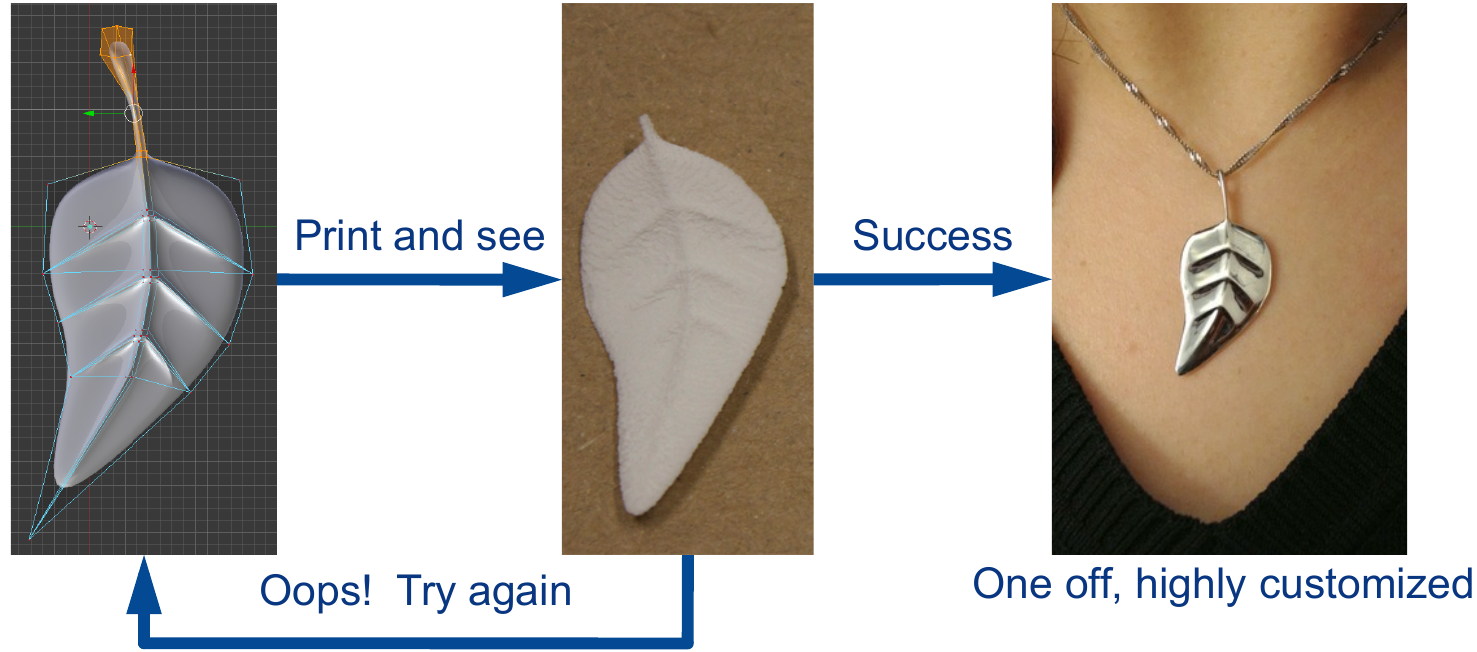
\includegraphics[width=\textwidth]{img/printing_pipeline}
  \end{figure}
\end{frame}

\begin{frame}
  \frametitle{Goal}
  \begin{figure}
    \centering
    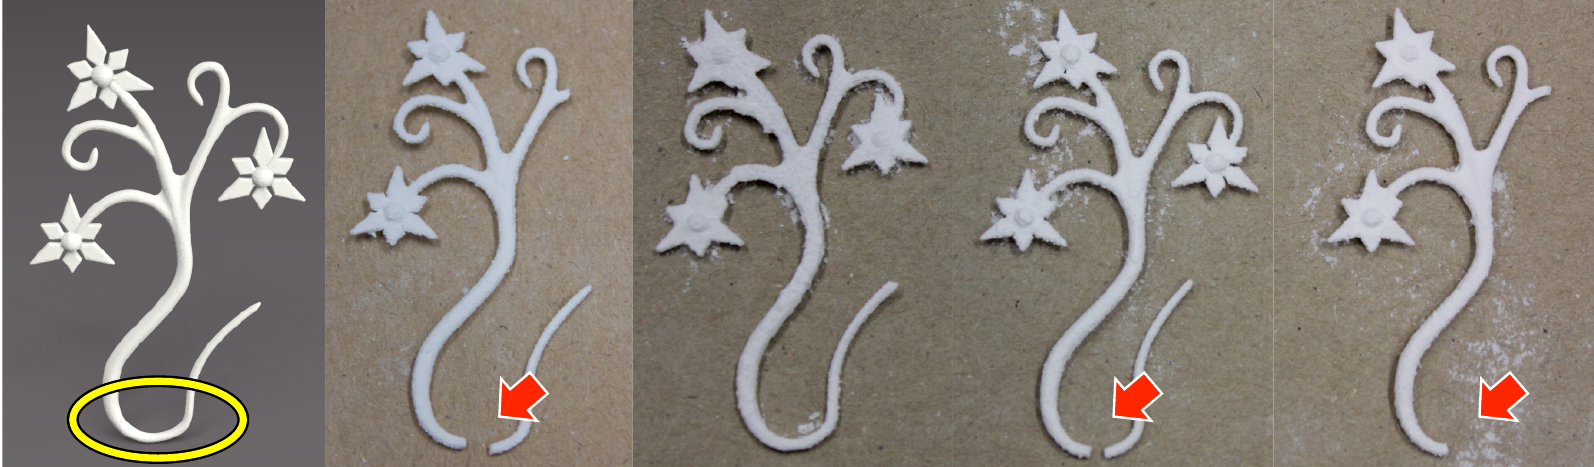
\includegraphics[width=\textwidth]{img/broken_flower}
  \end{figure}
  \pause
  \begin{itemize}
  \item Predict structure problems before 3D printing.
  \end{itemize}
\end{frame}

\begin{frame}
  \frametitle{Previous work}
  \begin{itemize}
  \item Stress relief
    \begin{figure}
      \centering
      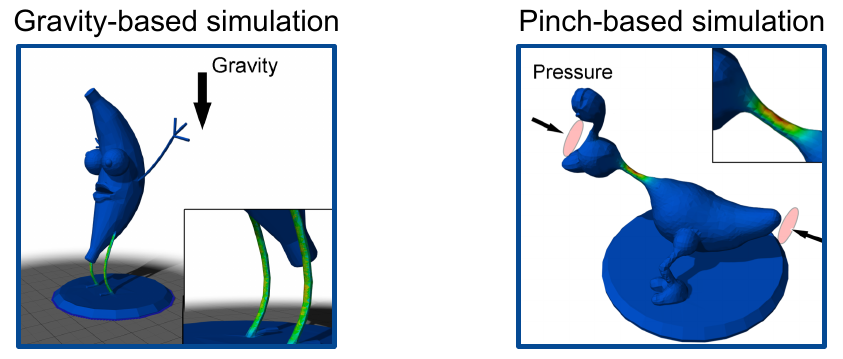
\includegraphics[width=0.8\textwidth]{img/stress_relief}
    \end{figure}
  \end{itemize}
  \TikzDraw {
  \visible<2-> {
    \node at (0, 0) {
      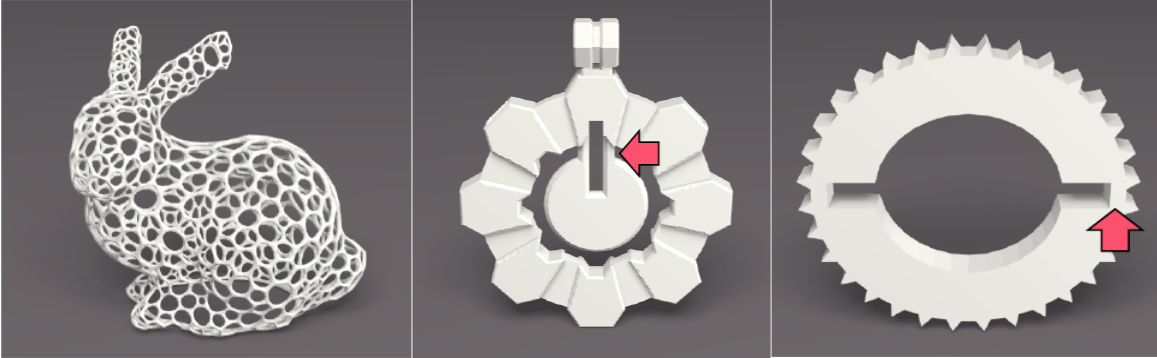
\includegraphics[width=\textwidth]{img/stress_relief_drawback}
    };
  }
  }
\end{frame}

\begin{frame}
  \frametitle{Idea}
  \begin{itemize}
  \item Apply stress test to check stress distribution
    \pause
  \item \TODO{What load causes the maximal damage?}
    \begin{figure}
    \centering
    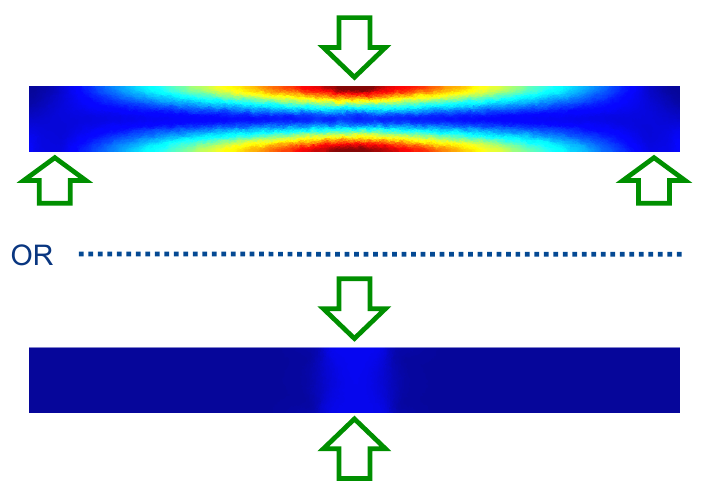
\includegraphics[width=0.7\textwidth]{img/load_on_beam}
    \end{figure}
  \end{itemize}
\end{frame}

\begin{frame}
  \frametitle{Formulation}
  \begin{itemize}
  \item Worst case formulation: maximize the largest stress under some parametric load
    \pause
    \begin{equation*}
      \boxed{
        \max_{x\in\Omega} \max_{F} \|\sigma(x, F) \|
        }
    \end{equation*}
    \pause
  \item Stress is calculated via linear elasticity
    \begin{equation*}
      \sigma = C:\epsilon
    \end{equation*}
    \pause
  \item \TODO{How to parameterize $F$?}
  \end{itemize}
\end{frame}

\begin{frame}
  \frametitle{Formulation}
  \begin{itemize}
  \item Surface force model
    \begin{itemize}
      \pause
    \item[-] Only positive normal forces are allowed: $F = pn$
      \pause
    \item[-] Bounded pressure: $p < p_{max}$
      \pause
    \item[-] Total intensity is fixed: $\int_{\partial \Omega} pdA  = F_{tot}$
      \pause
    \item[-] Eliminate global motion: $\int_{\partial\Omega} pndA= 0, \int_{\partial \Omega}pn\times (x-x_c)dA = 0$
    \end{itemize}
  \end{itemize}
\end{frame}

\begin{frame}
  \frametitle{Formulation}
  \begin{itemize}
  \item Find the worst case force distribution
    \begin{equation*}
      \begin{split}
        &\max_\Omega \max_p \|\sigma(u, p) \| \\
        &\ST \nabla\cdot \sigma  = 0 \text{ in } \Omega, \sigma\cdot n  = pn \text{ on } \partial \Omega, \\
        &\int_{\partial \Omega} pndA = 0, \int_{\partial\Omega} pn\times (x-x_c)dA = 0, \\
        &\int_{\Omega} u dV = 0, \int_{\Omega} u\times(x-x_c) dV = 0, \\
        & 0 \le p \le p_{max} \text{ on } \partial \Omega, \int_{\partial \Omega} pdA = F_{tot}.
      \end{split}
    \end{equation*}
    \pause
  \item Brute force method: impractical for usage
  \end{itemize}
\end{frame}

\begin{frame}
  \frametitle{Simplification}
  \begin{itemize}
  \item (I) Maximize stress of each of ``weak regions''
    \begin{equation*}
      \begin{split}
      &\max_{x \in \Omega} \max_{p} \|\sigma (x) \| \Rightarrow \\
      &\TODO{\max_{R\subset\Omega}} \max_{p} \TODO{\int_R} \|\sigma\| dV
      \end{split}
    \end{equation*}
    \begin{figure}
      \centering
      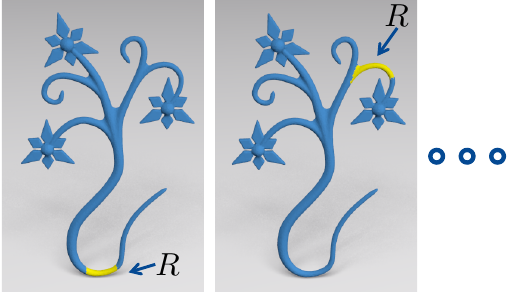
\includegraphics[width=0.5\textwidth]{img/weak_regions}
    \end{figure}
  \end{itemize}
\end{frame}

\begin{frame}
  \frametitle{Simplification}
  \begin{itemize}
  \item Find the ``weak region'' by solve linear modal analysis
    \begin{figure}
      \centering
      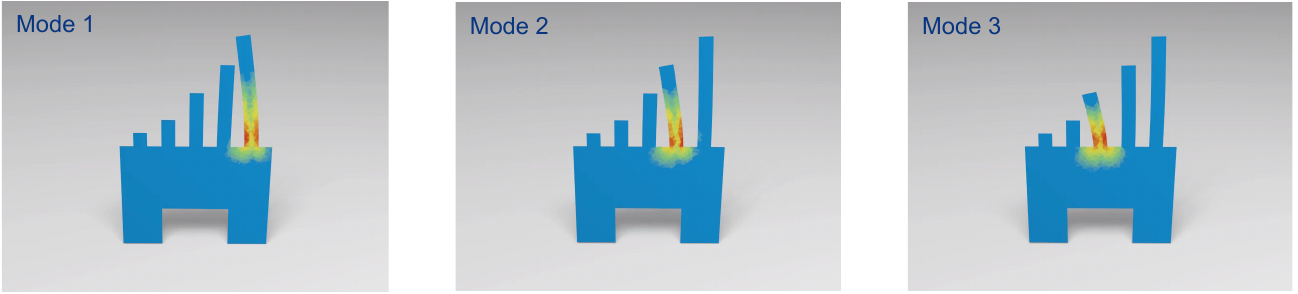
\includegraphics[width=0.9\textwidth]{img/lma_modes}
    \end{figure}
  \item Find the points with $1-\epsilon$ percentile largest stress, and
    extract the connected components.
    \pause
  \item \TODO{High stress with low energy}
  \end{itemize}
\end{frame}

\begin{frame}
  \frametitle{Simplification}
  \begin{itemize}
  \item (II) Approximate convex problem
    \begin{equation*}
      \begin{split}
        &\max_{p} \int_{R\subset \Omega} (\sigma_1^2+\sigma_2^2+\sigma_3^2)dV \Rightarrow \\
        &\max_{p} \int_{R\subset \Omega} \TODO{(\sigma_1+\sigma_2+\sigma_3)} dV \\
      \end{split}
    \end{equation*}
    \pause
  \item \TODO{Poor: $\sigma_1 \approx -\sigma_2$ or $\sigma_1 \approx -\sigma_3$}
  \item \TODOG{Good: $\sigma_1 \gg \sigma_2$ and $\sigma_1 \gg \sigma_3$}
  \end{itemize}  
\end{frame}

\begin{frame}
  \frametitle{Simplification}
  \begin{itemize}
  \item Over 36 models with various load $\frac{\sigma_1}{\sigma_1+\sigma_2+\sigma_3}$ average: 0.96
  \end{itemize}
  \begin{figure}
    \centering
    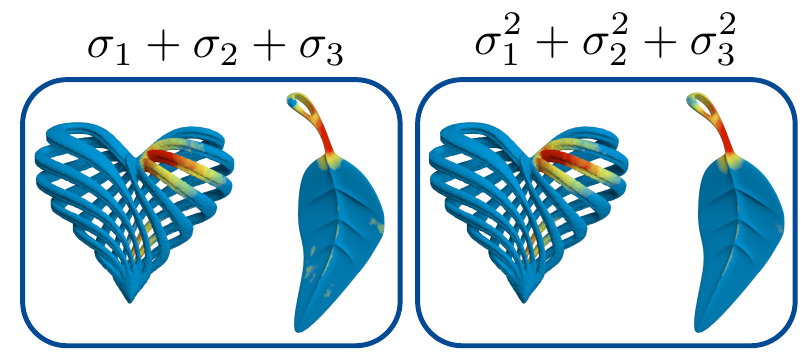
\includegraphics[width=\textwidth]{img/validation_trace}
  \end{figure}
\end{frame}

\begin{frame}
  \frametitle{Algorithm pipeline}
  \begin{figure}
    \centering
    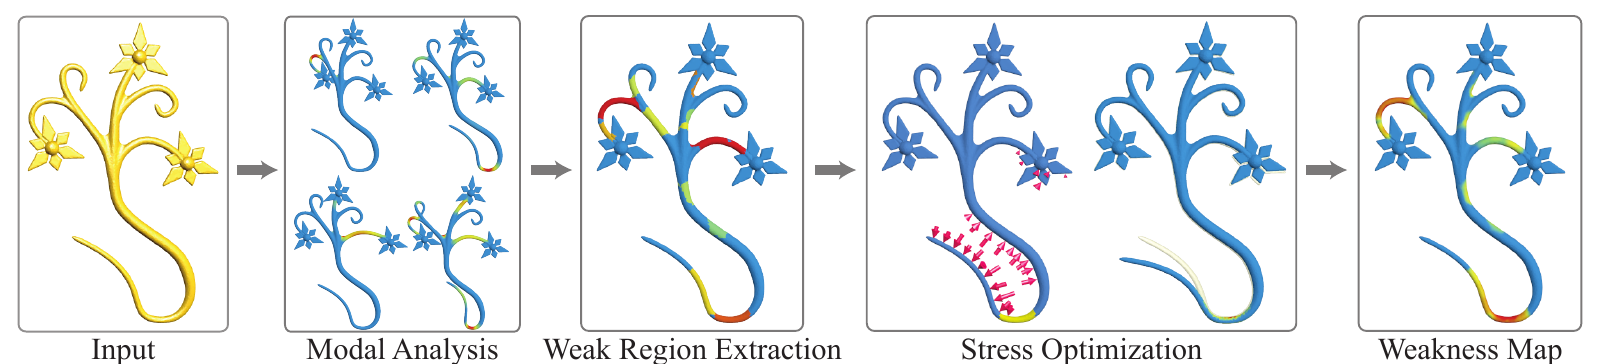
\includegraphics[width=\textwidth]{img/pipeline}
  \end{figure}
  \TODO{Weakness map: scalar field of maximal principle stress}
\end{frame}

\begin{frame}
  \frametitle{Results}
  \begin{figure}
    \centering
    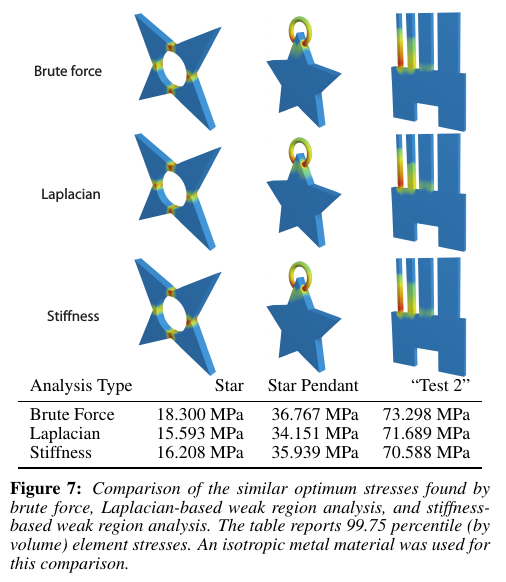
\includegraphics[width=0.6\textwidth]{img/comp_diff_methods}
  \end{figure}
\end{frame}

\begin{frame}
  \frametitle{Results}
  \begin{itemize}
  \item Weak region acceleration
    \begin{figure}
      \centering
      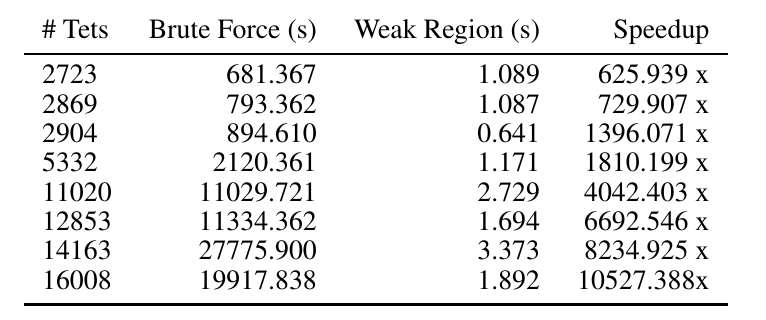
\includegraphics[width=0.9\textwidth]{img/timings}
    \end{figure}
  \end{itemize}
\end{frame}

\begin{frame}
  \frametitle{Results}
  \begin{figure}
    \centering
    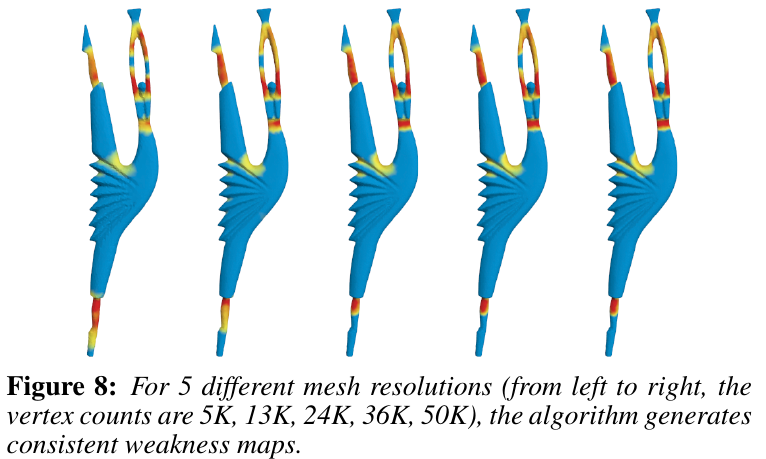
\includegraphics[width=\textwidth]{img/resolution}
  \end{figure}
\end{frame}

\begin{frame}
  \frametitle{Results}
  \begin{itemize}
  \item Drop test
    \begin{figure}
      \centering
      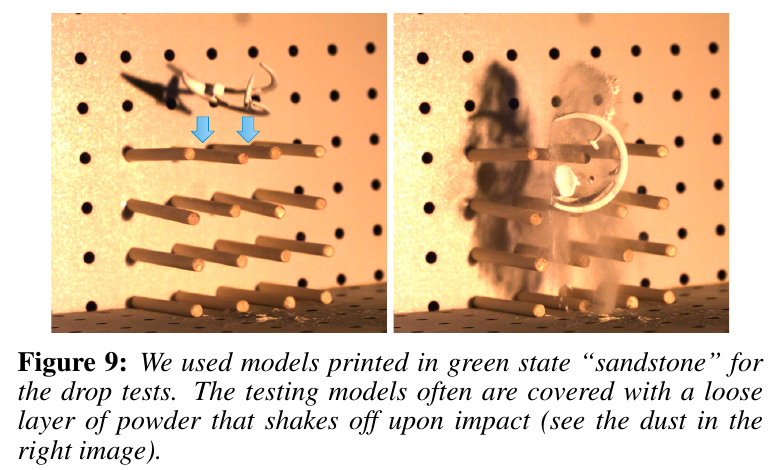
\includegraphics[width=0.9\textwidth]{img/drop_test}
    \end{figure}
  \end{itemize}
\end{frame}

\begin{frame}
  \frametitle{Results}
  \begin{figure}
    \centering
    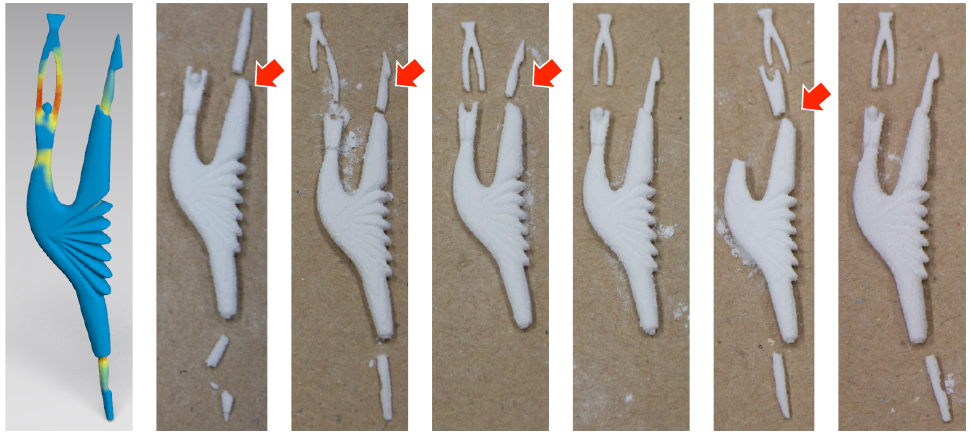
\includegraphics[width=\textwidth]{img/drop_dance}
  \end{figure}
\end{frame}

\begin{frame}
  \frametitle{Results}
  \begin{figure}
    \centering
    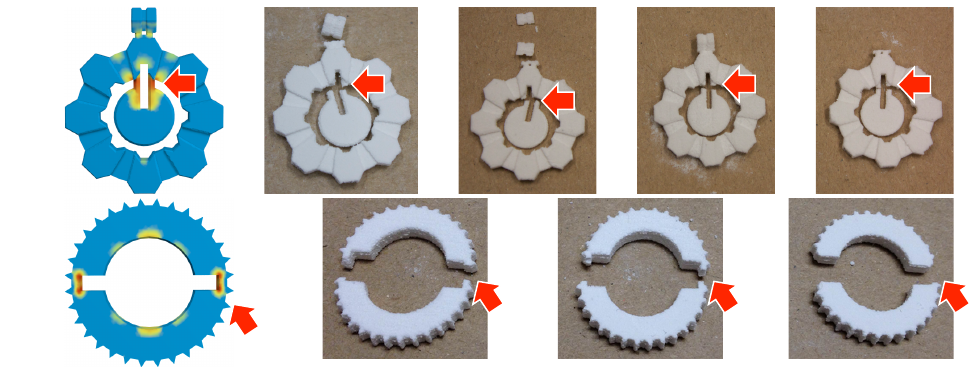
\includegraphics[width=\textwidth]{img/drop_nut}
  \end{figure}
\end{frame}

\begin{frame}
  \frametitle{Limitations}
  \begin{itemize}
  \item Linear elasticity.
  \item Complexity of real world material.
  \item Tet mesh generation.
  \item Structure improvement.
  \end{itemize}
\end{frame}

\begin{frame} 
  \TikzDraw {
    \node at (0, 0.5) {\Huge{Thanks!}};
  }
  %\gridlines
\end{frame}

\end{document}
